\documentclass[aspectratio=169,11pt]{beamer}
\usepackage[T1]{fontenc}
\usepackage[utf8]{inputenc}
\usepackage[brazilian]{babel}
\usepackage{lmodern,tikz,amsmath}
\usetikzlibrary{arrows.meta,positioning,calc}
\definecolor{Ink}{HTML}{17324D}
\definecolor{Teal}{HTML}{008C95}
\definecolor{Gold}{HTML}{E6A23C}
\definecolor{Paper}{HTML}{F5F8FA}
\definecolor{Muted}{HTML}{597184}
\setbeamercolor{normal text}{fg=Ink,bg=Paper}
\setbeamercolor{structure}{fg=Teal}
\setbeamercolor{block title}{fg=white,bg=Teal}
\setbeamercolor{block body}{fg=Ink,bg=white}
\setbeamertemplate{navigation symbols}{}
\setbeamersize{text margin left=9mm,text margin right=9mm}
\setbeamerfont{block title}{size=\normalsize,series=\bfseries}
\setbeamerfont{frametitle}{size=\Large,series=\bfseries}
\setbeamertemplate{frametitle}{\vspace{2mm}{\color{Teal}\scriptsize\insertsectionhead\par}\vspace{1mm}\insertframetitle\par}
\setbeamertemplate{footline}{\hspace{9mm}{\color{Muted}\tiny Gravidade, sinais e engenharia\hfill\insertframenumber\hspace{9mm}}\vspace{3mm}}
\newcommand{\key}[1]{\par\vspace{3mm}\begin{beamercolorbox}[sep=3mm,wd=\linewidth]{block body}\textbf{#1}\end{beamercolorbox}}
\newcommand{\src}[1]{\par\vspace{2mm}{\fontsize{8}{10}\selectfont\color{Muted}#1\par}}
\newcommand{\card}[2]{\begin{block}{#1}#2\end{block}}
\newcommand{\ring}[2]{\begin{tikzpicture}[scale=.85]\draw[Muted,dashed] (0,0) circle(1);\draw[Teal,very thick] (0,0) ellipse (#1 and #2);\foreach \a in {0,30,...,330}{\fill[Teal] ({#1*cos(\a)},{#2*sin(\a)}) circle(.055);}\end{tikzpicture}}
\title{E se a gravidade viajasse de outro jeito?}
\author{Gráviton de Souza}
\date{}
\begin{document}
\section{Uma conversa para quem pensa como engenheiro}
\begin{frame}{E se a gravidade viajasse de outro jeito?}
\begin{columns}\column{.64\textwidth}{\LARGE\bfseries Ondas, sensores e pistas sobre a gravidade}\par\vspace{5mm}Uma leitura acessível do TG de Wayne\par\vspace{5mm}{\color{Teal}Gráviton de Souza · ITA}\par\small Programa de Pós-Graduação em Física
\column{.30\textwidth}\centering\begin{tikzpicture}\foreach \r in {.4,.8,1.2,1.6}{\draw[Teal,line width=1.5pt] (0,0) circle(\r);}\fill[Gold] (0,0) circle(.13);\end{tikzpicture}\end{columns}\key{Não é preciso conhecer relatividade: vamos começar com ondas e medições.}
\end{frame}
\section{O mapa da conversa}
\begin{frame}{Três perguntas guiam a apresentação}
\card{1 · O que poderia mudar?}{A maneira como uma onda gravitacional viaja e deforma distâncias.}\card{2 · Como Wayne estudou isso?}{Escolheu um modelo e calculou suas consequências.}\card{3 · Como confiar numa medição?}{Separando o sinal físico dos efeitos do instrumento e da análise.}
\end{frame}
\section{Antes do TG: a intuição}
\begin{frame}{Uma onda transporta uma perturbação}
\begin{columns}\column{.56\textwidth}\begin{tikzpicture}[x=.8cm,y=1cm,>=Latex]\draw[Muted,->] (0,0)--(7,0);\draw[Teal,very thick,domain=0:6.5,samples=100] plot (\x,{.65*sin(100*\x)});\draw[Gold,thick,->] (4,1.2)--(6,1.2) node[midway,above]{propagação};\end{tikzpicture}\column{.40\textwidth}\card{Pense numa corda}{A forma da perturbação avança. Cada pequeno trecho oscila perto de sua posição.}\end{columns}\key{Frequência é o número de oscilações por segundo.}\src{Analogia para o conceito de onda; a gravidade não precisa de uma corda ou de um meio material.}
\end{frame}
\begin{frame}{Na gravidade, observamos mudanças de distância}
\begin{columns}\column{.46\textwidth}\centering\ring{1}{1}\par Antes da onda\column{.46\textwidth}\centering\ring{1.4}{.7}\par Em um instante da passagem\end{columns}\key{Partículas livres podem se aproximar numa direção e se afastar em outra.}\src{Desenho com deformação exagerada. O círculo tracejado é a referência.}
\end{frame}
\begin{frame}{Polarização é o desenho da deformação}
\begin{columns}\column{.30\textwidth}\centering\ring{1.3}{.7}\par\textbf{Estica aqui}\column{.30\textwidth}\centering\begin{tikzpicture}[rotate=45,scale=.85]\draw[Muted,dashed] (0,0) circle(1);\draw[Teal,very thick] (0,0) ellipse(1.3 and .7);\end{tikzpicture}\par\textbf{Estica na diagonal}\column{.30\textwidth}\card{Na relatividade geral}{Duas polarizações independentes descrevem essas deformações transversais.}\end{columns}\key{Assim como uma estrutura tem modos de vibração, uma onda tem padrões de deformação.}\src{Analogia de modos: o espaço não é uma estrutura elástica material.}
\end{frame}
\begin{frame}{E se o gráviton tivesse uma massa muito pequena?}
\card{Gráviton, em linguagem simples}{Nome dado ao quantum hipotético do campo gravitacional: uma ideia semelhante à relação entre luz e fótons.}\card{A pergunta estudada aqui}{Uma massa diferente de zero poderia mudar a propagação e os padrões de deformação previstos?}\key{O TG calcula ondas clássicas de uma teoria com massa; não observa partículas individuais.}
\end{frame}
\begin{frame}{Frequências diferentes podem viajar de modo diferente}
\begin{columns}\column{.58\textwidth}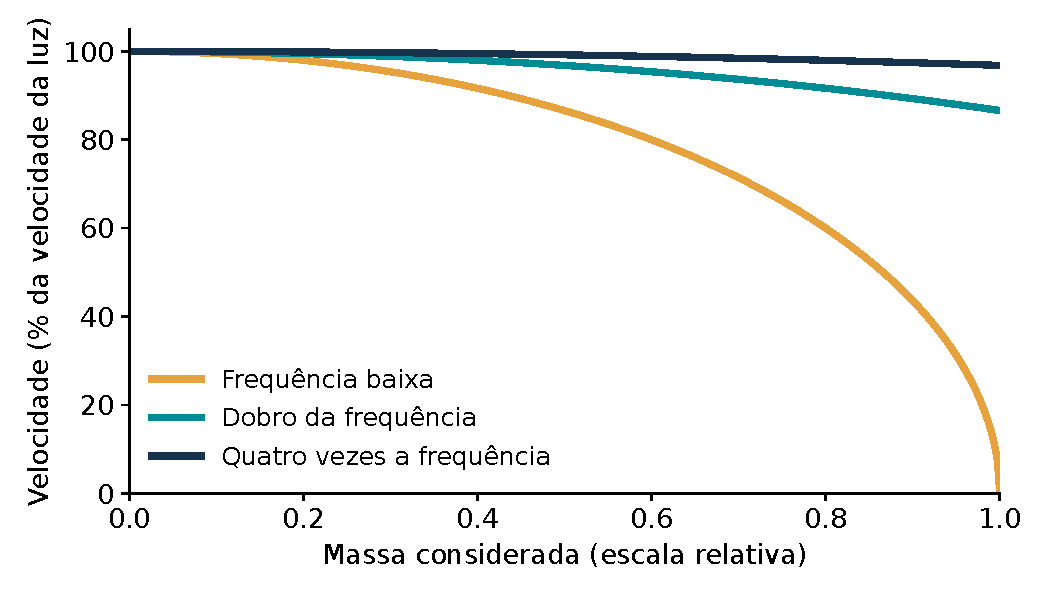
\includegraphics[width=\linewidth,height=.42\textheight,keepaspectratio]{dispersao_didatica.pdf}\column{.38\textwidth}\small\textbf{Leia apenas a tendência:}\par\vspace{3mm}Perto do limiar, o canal de menor frequência é mais afetado.\par\vspace{3mm}Os canais superiores permanecem mais próximos da velocidade da luz.\end{columns}\key{Dispersão: a velocidade de um pacote de onda depende de sua frequência.}\src{Ilustração analítica. Eixo horizontal: massa relativa à escala do primeiro canal; eixo vertical: velocidade relativa à luz.}
\end{frame}
\begin{frame}{O olhar da engenharia: modelo, entrada e resposta}
\centering\begin{tikzpicture}[>=Latex,node distance=8mm,b/.style={draw=Teal,fill=white,rounded corners,minimum height=17mm,text width=32mm,align=center}]\node[b](a){Onda\\incidente};\node[b,right=of a](b){Modelo\\da gravidade};\node[b,right=of b](c){Deformação\\prevista};\draw[->,thick](a)--(b);\draw[->,thick](b)--(c);\end{tikzpicture}\vspace{6mm}\card{Uma pergunta familiar}{Se eu mudar uma hipótese do modelo, a saída do sistema muda de um jeito que consigo reconhecer?}\key{Essa é uma boa porta de entrada para entender o TG.}
\end{frame}
\section{TG do Wayne for dummies}
\begin{frame}{TG do Wayne for dummies}
\leavevmode{\LARGE\bfseries Uma hipótese diferente.\par\vspace{4mm}Que assinatura ela deixaria?}\vspace{6mm}\card{O trabalho original}{Wayne Leonardo Silva de Paula\par\emph{Estados de polarização de ondas gravitacionais com gráviton massivo}\par ITA, 2003.}\src{Nesta seção, “Wayne” é o autor do TG original. A pesquisa posterior será apresentada separadamente.}
\end{frame}
\begin{frame}{A pergunta de Wayne, em uma frase}
\begin{block}{Se a gravidade tiver um termo de massa...}\Large ...a onda pode deformar um detector de maneiras diferentes das previstas por Einstein?\end{block}\vspace{5mm}\key{O objetivo era procurar assinaturas teóricas que ajudassem a distinguir modelos de gravidade.}\src{TG, capítulos 4 a 6.}
\end{frame}
\begin{frame}{Primeiro: escolher um problema que dê para resolver}
\card{Um modelo específico}{A teoria de Visser acrescenta um termo de massa e uma geometria de referência.}\card{Ondas pequenas}{Simplificar as equações mantendo a resposta de primeira ordem.}\card{Uma região pequena da frente de onda}{Tratar a onda como aproximadamente plana facilita identificar os padrões.}\src{TG, capítulos 4 e 5. As conclusões pertencem ao modelo e às aproximações adotadas.}
\end{frame}
\begin{frame}{Depois: transformar equações em movimento}
\centering\begin{tikzpicture}[>=Latex,node distance=5mm,b/.style={draw=Teal,fill=white,rounded corners,text width=28mm,minimum height=20mm,align=center,font=\small}]\node[b](a){Escrever a\\teoria};\node[b,right=of a](b){Simplificar\\a onda};\node[b,right=of b](c){Calcular\\a deformação};\node[b,right=of c](d){Comparar\\os padrões};\draw[->,thick](a)--(b);\draw[->,thick](b)--(c);\draw[->,thick](c)--(d);\end{tikzpicture}\vspace{5mm}\key{A matemática traduz uma hipótese sobre a gravidade em deslocamentos relativos.}\src{TG, capítulos 4 e 5 e apêndice Maple.}
\end{frame}
\begin{frame}{A “matriz” é uma tabela de resposta em três direções}
\begin{columns}\column{.40\textwidth}\centering\begin{tikzpicture}[>=Latex]\draw[->,very thick,Teal] (0,0)--(2,0) node[right]{direita};\draw[->,very thick,Teal] (0,0)--(0,1.8) node[above]{cima};\draw[->,very thick,Gold] (0,0)--(-1,-1) node[below]{frente};\end{tikzpicture}\column{.55\textwidth}\card{O que cada entrada informa?}{Como a separação entre duas partículas produz uma aceleração relativa numa dada direção.}\small Entradas cruzadas indicam que uma direção pode responder a uma separação em outra direção.\end{columns}\key{Pense numa tabela que liga a geometria inicial à tendência de deformação.}\src{No TG: componentes de maré da curvatura, reunidas na matriz elétrica do tensor de Riemann.}
\end{frame}
\begin{frame}{Que tipos de deformação entram nessa descrição?}
\begin{columns}[T]\column{.47\textwidth}\card{2 padrões transversais}{Estica numa direção e comprime na outra, com duas orientações.}\card{1 padrão de “respiração”}{Expande ou contrai o anel transversal.}\column{.47\textwidth}\card{2 padrões mistos}{Combinam deslocamentos laterais com a direção de propagação.}\card{1 padrão longitudinal}{Altera separações ao longo da propagação.}\end{columns}\key{Seis padrões geométricos possíveis não significam seis amplitudes livres em toda teoria.}\src{TG, figura 5.1 e capítulo 5; distinção com vínculos físicos discutida na dissertação, capítulo 3.}
\end{frame}
\begin{frame}{O computador ajudou a fazer a álgebra}
\begin{columns}[T]\column{.47\textwidth}\card{Ferramenta: Maple}{Manipular expressões simbólicas.\par\vspace{3mm}Calcular as componentes da resposta.\par\vspace{3mm}Comparar os dois modelos.}\column{.47\textwidth}\card{Uma verificação importante}{No caso da relatividade geral, o cálculo recuperou os dois padrões esperados.}\end{columns}\key{O computador executa as contas; as hipóteses e a interpretação continuam sendo parte da física.}\src{TG, página impressa 35 e apêndice A.}
\end{frame}
\begin{frame}{Onde procurar uma diferença pequena?}
\card{A pista encontrada}{Nas comparações do TG, os efeitos relativos associados à massa ganhavam importância em frequências menores.}\card{A conclusão histórica}{Entre os detectores analisados, Wayne apontou a faixa do LISA como promissora para distinguir os modelos.}\key{Escolher a faixa de frequência é parecido com escolher a banda de um sensor.}\src{TG, seções 6.2 e 6.3. A comparação teórica de amplitudes não calcula, sozinha, a detectabilidade.}
\end{frame}
\begin{frame}{O que Wayne entregou?}
\card{Uma previsão de padrões}{No modelo e tratamento históricos, encontrou até seis modos de polarização.}\card{Expressões para calcular a resposta}{Fórmulas que relacionam a onda à deformação de partículas de teste.}\card{Uma direção para investigar}{Examinar baixas frequências e a resposta dos detectores.}\src{TG, seção 6.3. O núcleo do trabalho foi publicado por de Paula, Miranda e Marinho em 2004.}
\end{frame}
\begin{frame}{Prever uma assinatura é o começo da medição}
\centering\begin{tikzpicture}[>=Latex,node distance=5mm,b/.style={draw=Teal,fill=white,text width=28mm,minimum height=18mm,align=center,font=\small}]\node[b](a){Previsão\\física};\node[b,right=of a](b){Resposta\\do sensor};\node[b,right=of b](c){Sinal\\e ruído};\node[b,right=of c](d){Conclusão\\estatística};\draw[->,thick](a)--(b);\draw[->,thick](b)--(c);\draw[->,thick](c)--(d);\end{tikzpicture}\vspace{5mm}\key{A pesquisa posterior pergunta: quanto dessa assinatura sobrevive até a conclusão?}
\end{frame}
\section{Da previsão à medição}
\begin{frame}{Pulsares funcionam como faróis cósmicos}
\begin{columns}\column{.54\textwidth}\centering\begin{tikzpicture}[>=Latex]\fill[Gold] (0,0) circle(.2);\node[below] at (0,-.25){Terra};\foreach \x/\y in {-2/1.6,2/1.6,2/-1.4}{\fill[Teal] (\x,\y) circle(.1);\draw[Teal,thick,->] (\x,\y)--(.2,0);}\node at (0,2.1){Pulsos vindos de pulsares};\end{tikzpicture}\column{.42\textwidth}\card{O que é um pulsar?}{Uma estrela de nêutrons em rotação, observada por seus pulsos periódicos.}\small Comparamos o horário previsto com o horário de chegada.\end{columns}\key{Uma rede de pulsares permite procurar alterações correlacionadas nos tempos de chegada.}
\end{frame}
\begin{frame}{Um atraso isolado pode ser ruído}
\card{Em um único pulsar}{Uma diferença no horário pode ter várias causas.}\card{Em vários pulsares}{O padrão conjunto ajuda a separar efeitos comuns e individuais.}\card{A geometria importa}{Pulsares em direções diferentes respondem de maneiras relacionadas à mesma perturbação.}\key{Como em uma rede de sensores: o desenho da correlação também é informação.}
\end{frame}
\begin{frame}{Resumir dados pode esconder uma diferença}
\begin{columns}\column{.47\textwidth}\card{Medição detalhada}{Temperaturas: 20, 30 e 40 °C.\par\vspace{2mm}Outro sistema: 30, 30 e 30 °C.}\column{.47\textwidth}\card{A mesma média}{Ambos têm média de 30 °C.\par\vspace{2mm}Mas só um tem um gradiente.}\end{columns}\key{Na pesquisa, resumir frequências pode apagar parte do padrão que distingue os modelos.}\src{Exemplo didático inventado, sem relação numérica com as simulações da dissertação.}
\end{frame}
\begin{frame}{Como testar a análise sem conhecer o Universo?}
\card{1 · Criar um sinal com resposta conhecida}{Escolhemos os parâmetros verdadeiros da simulação.}\card{2 · Acrescentar ruído e analisar}{Aplicamos métodos diferentes à mesma realização.}\card{3 · Repetir e comparar}{Verificamos se os métodos recuperam a verdade com a frequência esperada.}\key{É o equivalente estatístico de calibrar um instrumento com uma referência conhecida.}
\end{frame}
\section{O que aprendemos com a pesquisa posterior}
\begin{frame}{“90\%” no relatório precisa funcionar no teste}
\begin{columns}\column{.52\textwidth}\centering\begin{tikzpicture}[x=.047cm,y=1cm]\fill[Teal] (0,1) rectangle (90,1.5);\node[anchor=west] at (0,1.9){\small Referência nominal: 90\%};\fill[Gold] (0,-.5) rectangle (62.6,0);\node[anchor=west] at (0,.4){\small Resultado: cerca de 63\%};\end{tikzpicture}\column{.43\textwidth}\card{Um resultado concreto}{Um método aproximado incluiu o valor verdadeiro em 313 de 500 testes, para um parâmetro de ruído.}\end{columns}\key{Conhecer a média e a variância não garante uma boa descrição dos dados.}\src{Dissertação, cap. 6: EFAC em $A_{\rm CN}$, cobertura central nominal de 90\%. Contagem nominal; sensibilidade numérica: 299 a 325 casos.}
\end{frame}
\begin{frame}{Uma faixa estreita pode vir da escolha inicial}
\card{Experimento mental}{Antes de medir, aceitamos valores entre 0 e 100, todos igualmente plausíveis.}\card{Se a medição não informar nada...}{O limite que deixa 95\% da probabilidade abaixo dele continua sendo 95.}\key{O número “95” veio da regra inicial. Ele não demonstra aprendizado com os dados.}\src{Analogia da priori uniforme: na dissertação, a variável de massa vai de 0 a 1 e o limite sem informação é 0,95.}
\end{frame}
\begin{frame}{Usar uma frequência para representar todas funciona?}
\card{Um teste controlado}{Em 50 casos, com parâmetros auxiliares fixados, as diferenças médias do limite ficaram dentro de 1\% da faixa de massa adotada.}\card{O alcance da resposta}{Ao estimar também os parâmetros auxiliares, a comparação mais ampla permaneceu inconclusiva.}\key{A aproximação passou por um teste específico; sua validade depende das condições da análise.}\src{Dissertação: contrastes condicionais B/C e comparação marginalizada. “1\%” refere-se à largura da priori, não a um erro relativo da massa.}
\end{frame}
\begin{frame}{Corrigir o relógio também modifica o sinal}
\begin{columns}\column{.47\textwidth}\card{Pense numa régua com tendência}{Ao remover uma inclinação do registro, também removemos qualquer sinal parecido com essa inclinação.}\column{.47\textwidth}\card{Nos pulsares}{Ajustar rotação e termos anuais pode reduzir potência em certas frequências e ligar canais antes separados.}\end{columns}\key{A análise deve incluir o efeito do próprio ajuste, como fazemos ao caracterizar um filtro.}\src{Experimento sintético de timing da dissertação; não é uma análise de tempos de chegada observados.}
\end{frame}
\section{A ideia que fica}
\begin{frame}{Duas contribuições, uma mesma lógica}
\begin{columns}[T]\column{.47\textwidth}\card{Wayne: prever a assinatura}{Uma hipótese diferente de gravidade pode produzir padrões diferentes de deformação.}\column{.47\textwidth}\card{Pesquisa posterior: testar a leitura}{Instrumento, resumo dos dados e modelo estatístico influenciam o que conseguimos concluir.}\end{columns}\key{Boa ciência liga uma hipótese física a uma medição que foi testada e compreendida.}
\end{frame}
\begin{frame}{Se você lembrar de apenas três coisas...}
\card{Ondas têm padrões}{Polarização é a forma da deformação.}\card{Modelos fazem previsões}{Wayne calculou como uma hipótese de massa mudaria esses padrões.}\card{Números precisam de contexto}{Uma conclusão depende do sensor, do ruído e da maneira de analisar.}\vspace{2mm}{\color{Teal}\Large Obrigado! Vamos às perguntas.}
\end{frame}
\appendix
\section{Apoio à conversa}
\begin{frame}{Um pequeno dicionário, sem fórmulas}
\small
\card{Polarização e dispersão}{Polarização: desenho da deformação. Dispersão: dependência da velocidade com a frequência.}
\card{Ruído e calibração}{Ruído: variações que dificultam a inferência do sinal. Calibração: conferir se um método se comporta como promete.}
\card{Priori e posterior}{Priori: distribuição adotada antes dos dados. Posterior: distribuição obtida ao combinar essa escolha com os dados e o modelo.}
\end{frame}
\begin{frame}{Para continuar a conversa}
\card{O ponto de partida}{Wayne Leonardo Silva de Paula. \emph{Estados de polarização de ondas gravitacionais com gráviton massivo}. TG, ITA, 2003. Capítulos 4--6 e apêndice A.}
\card{O artigo histórico}{de Paula, Miranda e Marinho. \emph{Polarization states of gravitational waves with a massive graviton}. Classical and Quantum Gravity, 2004.}
\card{A pesquisa posterior e os materiais}{Dissertação de Gráviton de Souza, ITA. Fundamentos, simulações e limites dos métodos.\par\href{https://github.com/flavioluiz/TGdoWayne}{github.com/flavioluiz/TGdoWayne}}
\end{frame}
\end{document}
